% B.Tech project report, NIT Warangal.
% Layout follows the institute's LaTeX thesis template (Template_for_Thesis, 2024):
% A4, Computer Modern 12 pt, 1.5 spacing, 30/20 mm side margins, left-aligned
% chapter heads, blue hyperlinks, author-year references, appendices after them.
% Compiles on Overleaf with pdfLaTeX + BibTeX. Figures and numbers in figures/ and
% generated/ are copied in by scripts/make_paper_figures.py; do not edit them by hand.
\documentclass[12pt,a4paper,oneside,openany]{report}

\usepackage[a4paper,left=30mm,right=20mm,top=30mm,bottom=25mm,
            headheight=15pt,headsep=8mm,footskip=12mm]{geometry}
\usepackage{amsmath,amssymb}
\usepackage[T1]{fontenc}
\usepackage{setspace}
\setstretch{1.5}

\usepackage{graphicx}
\graphicspath{{figures/}}
\usepackage{booktabs,tabularx,array,longtable}
\usepackage{xcolor}
\usepackage{tikz}
\usetikzlibrary{positioning,arrows.meta}
\usepackage[font=small,labelfont=bf,labelsep=space]{caption}
\usepackage{enumitem}
\usepackage{titlesec}
\usepackage{indentfirst} % the template indents the first paragraph after a heading
\usepackage{fancyhdr}
\usepackage[square,sort,comma]{natbib}
\usepackage[colorlinks=true,linkcolor=blue,citecolor=blue,urlcolor=blue]{hyperref}

% ---------------------------------------------------------------------------
% Fill in these details once; every front-matter page reads them.
% ---------------------------------------------------------------------------
\newcommand{\ProjectTitle}{Byzantine-Resilient Federated Learning for Tactical UAV Swarms over Lossy Wireless Links}

% Students: name and roll number, one \Student line each.
\newcommand{\StudentList}{%
  \Student{Nasika Sasank}{23ECB0A03}%
  \Student{Aaron George}{23ECB0F06}%
  \Student{Sachin Sreekumar Nair}{23ECB0F11}%
}

\newcommand{\Supervisor}{Dr.~Chayan Bhar}
\newcommand{\SupervisorDesignation}{Assistant Professor}
\newcommand{\HOD}{Prof.~Ravi Kumar Jatoth}
\newcommand{\Department}{Department of Electronics and Communication Engineering}
\newcommand{\Program}{Electronics and Communication Engineering}
\newcommand{\Degree}{Bachelor of Technology}
\newcommand{\SubmissionMonth}{November}
\newcommand{\SubmissionYear}{2026}
\newcommand{\AcademicYear}{2026--2027}
\newcommand{\Place}{Warangal}

% Generated by scripts/make_paper_figures.py -- do not edit by hand.
\newcommand{\NumRuns}{720}
\newcommand{\NumSeeds}{10}
\newcommand{\PdrTrace}{99.8}
\newcommand{\PdrStress}{65.0}
\newcommand{\TelGain}{-3.5}
\newcommand{\TelLo}{-5.1}
\newcommand{\TelHi}{-2.1}
\newcommand{\MaskGain}{4.2}
\newcommand{\MaskLo}{2.2}
\newcommand{\MaskHi}{5.9}
\newcommand{\PrimGain}{-2.7}
\newcommand{\PrimLo}{-3.9}
\newcommand{\PrimHi}{-1.5}
\newcommand{\AccCcraStress}{46.0}
\newcommand{\AccMaskStress}{49.5}
\newcommand{\AccNoctxStress}{45.3}
\newcommand{\AccFltrustStress}{50.1}
\newcommand{\RejCcra}{41.2}
\newcommand{\RejMask}{13.8}
\newcommand{\AccptCcra}{8.8}
\newcommand{\AccptMask}{13.5}
\newcommand{\RejFltrust}{4.8}
\newcommand{\VsFltTrace}{2.6}
\newcommand{\VsFltTraceLo}{0.9}
\newcommand{\VsFltTraceHi}{4.5}
\newcommand{\VsFltStress}{-0.6}
\newcommand{\VsFltStressLo}{-2.0}
\newcommand{\VsFltStressHi}{1.0}
\newcommand{\DivFedavg}{41}
\newcommand{\DivMedian}{26}
\newcommand{\AllMask}{52.8}
\newcommand{\AllFedavg}{37.3}

% Generated by scripts/make_paper_figures.py; do not edit.
\newcommand{\BpNumRuns}{240}
\newcommand{\NumCombinedRuns}{960}
\newcommand{\BpDivFresh}{41}
\newcommand{\BpAllFresh}{37.7}
\newcommand{\BpCleanStressFresh}{56.9}
\newcommand{\BpAttackStressFresh}{30.3}
\newcommand{\BpDivReuse}{42}
\newcommand{\BpAllReuse}{36.4}
\newcommand{\BpCleanStressReuse}{51.5}
\newcommand{\BpAttackStressReuse}{26.9}
\newcommand{\BpCleanGain}{5.4}
\newcommand{\BpCleanLo}{4.1}
\newcommand{\BpCleanHi}{6.7}
\newcommand{\BpAttackGain}{3.4}
\newcommand{\BpAttackLo}{0.9}
\newcommand{\BpAttackHi}{6.6}
\newcommand{\VsBpAttack}{19.2}
\newcommand{\VsBpAttackLo}{15.9}
\newcommand{\VsBpAttackHi}{23.0}
\newcommand{\VsBpClean}{-2.1}
\newcommand{\VsBpCleanLo}{-2.9}
\newcommand{\VsBpCleanHi}{-1.4}
\newcommand{\AccMaskCleanStress}{54.7}
\newcommand{\FltVsBpAttack}{19.8}
\newcommand{\IdealHandovers}{43.5}
\newcommand{\TraceHandovers}{0.7}
\newcommand{\XcheckMax}{1.1}
\newcommand{\XcheckMean}{0.3}
\newcommand{\XcheckRuns}{24}


% Paragraphs: 10 mm indent, a little space between paragraphs (as in the template).
\setlength{\parindent}{10mm}
\setlength{\parskip}{7pt}
\setlength{\emergencystretch}{2em} % lets lines with unbreakable file names wrap cleanly

% Chapter heads: "Chapter N" and the title on separate lines, left-aligned, bold.
% Unnumbered heads (Contents, Abstract, References, ...) sit at the same height.
\newlength{\ChapterTop}\setlength{\ChapterTop}{55.5pt}
\titleformat{\chapter}[display]{\Large\bfseries}{\chaptertitlename\ \thechapter}{25.6pt}{\Large}
\titleformat{name=\chapter,numberless}[block]{\Large\bfseries}{}{0pt}{\Large}
\titlespacing{\chapter}{0pt}{\ChapterTop}{24.5pt}
\titleformat{\section}{\large\bfseries}{\thesection}{1em}{}
\titleformat{\subsection}{\normalsize\bfseries}{\thesubsection}{1em}{}
\setcounter{secnumdepth}{2}
\setcounter{tocdepth}{2}
\titleformat{\subsubsection}[runin]{\normalsize\bfseries\itshape}{}{0pt}{}[.]

% Running head on continuation pages: chapter title left, page number right,
% rules above and below; chapter-opening pages show the number centred.
\pagestyle{fancy}
\fancyhf{}
\fancyhead[L]{\nouppercase{\leftmark}}
\fancyhead[R]{\thepage}
\renewcommand{\headrulewidth}{0.4pt}
\renewcommand{\footrulewidth}{0.4pt}
\renewcommand{\chaptermark}[1]{\markboth{#1}{}}
\fancypagestyle{plain}{\fancyhf{}\fancyfoot[C]{\thepage}%
  \renewcommand{\headrulewidth}{0pt}\renewcommand{\footrulewidth}{0pt}}

\renewcommand{\bibname}{References}
\renewcommand{\contentsname}{Contents}

% Numbers used in prose.
\newcommand{\pp}{\,pp}
\newcommand{\ci}[2]{$[#1,\,#2]$}
\newcommand{\Student}[2]{#1 & #2 \\}
% Unnumbered front-matter chapter that still appears in the contents.
\newcommand{\FrontChapter}[1]{\chapter*{#1}\addcontentsline{toc}{chapter}{#1}\markboth{#1}{#1}}

\begin{document}

% ---------------------------------------------------------------- front matter
\pagenumbering{roman}
% Title page, laid out as in the institute template (page i, no number shown).
\begin{titlepage}
\centering
\setstretch{1.2}
{\Large\bfseries \MakeUppercase{\ProjectTitle}\par}
\vspace{12mm}
{\bfseries\itshape Project report submitted to the\\
National Institute of Technology Warangal\\
For award of the degree\par}
\vspace{3mm}
{\bfseries\itshape of\par}
\vspace{2mm}
{\large\bfseries \Degree\par}
{\large\bfseries in \Program\par}
\vspace{2mm}
{\large\bfseries\itshape by\par}
\vspace{3mm}
{\large\bfseries
\begin{tabular}{l@{\hspace{10mm}}l}
\StudentList
\end{tabular}\par}
\vspace{4mm}
{\large Under the guidance of\par}
\vspace{1mm}
{\large\bfseries \Supervisor\par}
\vfill
\IfFileExists{figures/nitw_logo.jpg}{
\includegraphics[height=42mm]{nitw_logo.jpg}\par}{}
\vfill
{\large\bfseries \MakeUppercase{\Department}\\
NATIONAL INSTITUTE OF TECHNOLOGY WARANGAL\\
\SubmissionMonth\ \SubmissionYear\par}
\end{titlepage}
         % i
% Approval of the viva-voce board (template page ii; listed as "Certificate of Approval").
\clearpage
\setcounter{page}{2}
\thispagestyle{empty}
\phantomsection\addcontentsline{toc}{chapter}{Certificate of Approval}
\begin{center}
\textbf{APPROVAL OF THE VIVA-VOCE BOARD}
\end{center}
\vspace{4mm}
\hfill DD/MM/YYYY

\vspace{6mm}
{\sloppy
Certified that the project report entitled \MakeUppercase{\ProjectTitle} submitted by
{\renewcommand{\Student}[2]{\StudentSep\MakeUppercase{#1} (#2)\def\StudentSep{, }}\def\StudentSep{}\StudentList}
to the National Institute of Technology, Warangal, for the award of the degree of
\Degree{} in \Program{} has been accepted by the examiners and that the students have
successfully defended the work in the viva-voce examination held today.\par}

\vspace{30mm}
\noindent(Examiner)\hfill(Examiner)\hfill(Examiner)

\vspace{30mm}
\noindent(Supervisor)\hfill(Head of the Department)

\vspace{30mm}
\noindent\hfill(Chairman)
      % ii  Certificate of Approval
% Certificate (template page iii), to be printed on the departmental letterhead.
\clearpage
\thispagestyle{plain}
\phantomsection\addcontentsline{toc}{chapter}{Certificate}
\begin{center}
\textbf{\underline{CERTIFICATE}}
\end{center}
\vspace{4mm}

{\sloppy\noindent
This is to certify that the project report entitled \textbf{\ProjectTitle}, submitted by
{\renewcommand{\Student}[2]{\StudentSep\textbf{#1} (#2)\def\StudentSep{, }}\def\StudentSep{}\StudentList}
to the National Institute of Technology Warangal, is a record of bona fide work carried
out under my supervision in the \Department{} during the academic year \AcademicYear,
and I consider it worthy of consideration for the award of the degree of \Degree{} in
\Program{} of the Institute.\par}

\vspace{30mm}
\noindent
\begin{tabularx}{\textwidth}{@{}>{\centering\arraybackslash}X >{\centering\arraybackslash}X@{}}
\rule{50mm}{0.4pt} & \rule{50mm}{0.4pt} \\
\Supervisor & \HOD \\
Supervisor & Head of the Department \\
\end{tabularx}

\vspace{12mm}
\noindent Date:
   % iii
% Declaration (template page iv).
\clearpage
\thispagestyle{empty}
\phantomsection\addcontentsline{toc}{chapter}{Declaration}
\noindent\hspace{10mm}\textbf{DECLARATION}

\vspace{10mm}
\noindent\hspace{10mm}We certify that
\begin{enumerate}[label=\alph*., leftmargin=8mm, itemsep=2pt]
\item The work contained in this report is original and has been done by us under the
  general supervision of our supervisor.
\item The work has not been submitted to any other Institute for any degree or diploma.
\item We have followed the guidelines provided by the Institute in writing the report.
\item Whenever we have used materials (data, theoretical analysis, and text) from other
  sources, we have given due credit to them by citing them in the text of the report and
  giving their details in the references.
\item Whenever we have quoted written materials from other sources, we have put them
  under quotation marks and given due credit to the sources by citing them and giving
  required details in the references.
\end{enumerate}

\vspace{22mm}
\noindent
{\renewcommand{\Student}[2]{%
  \begin{minipage}[t]{0.32\textwidth}\centering
  \rule{40mm}{0.4pt}\\#1\\#2
  \end{minipage}\hfill}%
\StudentList}

\vspace{4mm}
\hfill Signature of the Students
   % iv
% Acknowledgements (template page v, before the abstract).
\FrontChapter{Acknowledgements}
\thispagestyle{empty}

We thank our supervisor, \Supervisor, for steering this project towards realistic
wireless conditions and fair, like-for-like comparisons, and for asking us to state our
findings with the evidence behind them. We thank the Head of the Department, \HOD, and
the faculty of the \Department{} for their support. We also thank the creators of the
DeepSense~6G dataset for making their UAV measurements available.

\vspace{10mm}
\begin{flushright}
{\renewcommand{\Student}[2]{\textbf{#1}\\}\StudentList}
\end{flushright}
 % v
% 3.7: abstract, at most 500 words.
\FrontChapter{Abstract}
\thispagestyle{empty}

Swarms of unmanned aerial vehicles (UAVs) can learn a shared perception model with
federated learning (FL): each UAV trains on the images it collects and sends only a
model update to a ground base station. In a tactical setting two problems arise
together. Air-to-ground links lose packets because of fading, distance, handover and
jamming, and some UAVs may be captured and made to send poisoned updates. Most
Byzantine-robust aggregation rules assume that every update arrives intact, while
most work on FL over unreliable links assumes that every client is honest. This
project studies both problems in one system.

We built a simulation framework in PyTorch for hierarchical FL over a UAV swarm. Ten
UAVs with non-identically distributed aerial images are served by three base
stations, which aggregate locally and synchronize every five rounds. Uplink packet
losses come either from a synthetic channel with path loss, Rayleigh fading and a
ground jammer, or from a measured UAV received-power trace (DeepSense~6G Scenario~23)
replayed at a chosen signal-to-noise ratio. Three of the UAVs mount sign-flip,
ALIE-style or inner-product-manipulation attacks. The framework includes FedAvg,
coordinate-wise median, FLTrust, a cosine-weighted rule taken from prior UAV-FL
work, and a reputation-based aggregator, CCRA, that we designed. CCRA compares each
update with a reference update computed on a small trusted dataset, keeps a
reputation for every UAV across rounds, and can use link information in two ways:
by ignoring coordinates whose packets were lost (erasure masking), and by letting
link telemetry slow down how fast a UAV regains trust.

The work proceeded in three phases. A FedAvg baseline reached
62.6\% (IID) and 60.2\% (non-IID) test accuracy. A preliminary single-seed study
suggested that CCRA resisted a label-flipping attack better than the cosine-weighted
baseline. To test which part of CCRA was responsible, we then ran a controlled,
prespecified study of \NumRuns{} training runs on an A100 GPU: \NumSeeds{} paired
seeds, four attack settings, three channel conditions and six aggregators. Diverged
runs were scored at chance rather than discarded, and all uncertainty was estimated
with a paired bootstrap over seeds.

The study gave a clear and partly negative answer. On a weak (5\,dB) link under
attack, erasure masking improved accuracy by \MaskGain{} percentage points (95\%
confidence interval \ci{\MaskLo}{\MaskHi}). Adding link telemetry to the reputation
update changed accuracy by \TelGain{} points (\ci{\TelLo}{\TelHi}) because it
rejected \RejCcra\% of honest updates, against \RejMask\% without telemetry. We
explain this with a short analysis of the reputation rule: when rewards are slowed
but penalties are not, an honest UAV's reputation settles near its worst rounds. All
reference-based aggregators avoided divergence, whereas FedAvg and the median
diverged in \DivFedavg{} and \DivMedian{} of 120 runs.

The result changes the direction of the project. The useful channel-aware component
is erasure masking, and the reputation reward rule must be redesigned before link
telemetry can help. The findings are written up as a four-page letter in IEEE format.
The second phase will revise the reward rule, test it on fresh seeds and
higher-mobility traces, and evaluate adaptive attackers.

\textbf{Index Terms :} Federated learning, UAV swarm, Byzantine robustness,
packet erasure, hierarchical aggregation, reputation.
      % vi

\clearpage
\markboth{Contents}{Contents}
\tableofcontents
\clearpage
\phantomsection\addcontentsline{toc}{chapter}{List of Figures}
\markboth{List of Figures}{List of Figures}
\listoffigures
\clearpage
\phantomsection\addcontentsline{toc}{chapter}{List of Tables}
\markboth{List of Tables}{List of Tables}
\listoftables
% List of abbreviations (template page xi), then the symbols used.
\FrontChapter{List of Abbreviations}
\thispagestyle{empty}

\begin{longtable}{@{\hspace{12mm}}p{28mm}p{114mm}@{}}
ALIE & A Little Is Enough (model-poisoning attack) \\
BS & Base station \\
CCRA & Context-Calibrated Robust Aggregation (the aggregator studied here) \\
CI & Confidence interval \\
CNN & Convolutional neural network \\
CosAvg & Cosine-similarity weighted averaging \\
EMA & Exponential moving average \\
EW & Electronic warfare \\
FedAvg & Federated averaging \\
FL & Federated learning \\
HFL & Hierarchical federated learning \\
IID & Independent and identically distributed \\
IPM & Inner-product manipulation (model-poisoning attack) \\
PDR & Packet delivery ratio \\
PER & Packet error rate \\
pp & Percentage points \\
RMS & Root mean square \\
SGD & Stochastic gradient descent \\
SINR & Signal-to-interference-plus-noise ratio \\
SNR & Signal-to-noise ratio \\
TEE & Trusted execution environment \\
UAV & Unmanned aerial vehicle \\
\end{longtable}

\FrontChapter{List of Symbols}
\thispagestyle{empty}

\begin{longtable}{@{\hspace{12mm}}p{28mm}p{114mm}@{}}
$K$ & Number of UAVs (clients) \\
$B$ & Number of base stations \\
$E$ & Edge rounds between global synchronizations \\
$P$ & Number of model parameters \\
$L$ & Parameters per packet \\
$f$ & Number of Byzantine UAVs \\
$\mathcal{D}_k$, $n_k$ & Local dataset of UAV $k$ and its size \\
$\mathcal{D}_0$ & Trusted root dataset held by each base station \\
$\mathbf{w}^t$, $\mathbf{w}^t_b$ & Global model and edge model of BS $b$ in round $t$ \\
$\boldsymbol{\Delta}_k^t$ & Model update sent by UAV $k$ in round $t$ \\
$\mathbf{m}_k$ & Delivery mask: 1 where the packet carrying a coordinate arrived \\
$\mathbf{r}$ & Reference update computed on $\mathcal{D}_0$ \\
$\gamma_k$, $\bar\gamma$ & Uplink SNR of UAV $k$; reference SNR of the trace \\
$p_k$ & Packet error probability of UAV $k$ \\
$a$, $\gamma_{\mathrm{th}}$ & Slope and threshold of the packet-error curve \\
$s_k$ & Norm-clipping factor \\
$c_k$ & Masked cosine similarity to the reference update \\
$b_k$ & Behaviour score in $[0,1]$ \\
$T_k$ & Reputation (trust) of UAV $k$ \\
$e_k$ & Link evidence in $[0,1]$ that slows reputation rewards \\
$\beta$, $\tau$ & Reputation memory and exclusion gate \\
$\omega_k$ & Aggregation weight of UAV $k$ \\
$\alpha$ & Dirichlet concentration of the non-IID data split \\
$\lambda$, $z$, $\epsilon$ & Strengths of the sign-flip, ALIE and IPM attacks \\
\end{longtable}


% ---------------------------------------------------------------- main text
\clearpage
\pagenumbering{arabic}
\chapter{Introduction}
\thispagestyle{plain}
\label{ch:intro}

\section{Background}
Small unmanned aerial vehicles (UAVs) are now used in groups, or swarms, for
surveillance, search and rescue, disaster assessment and border patrol. Each UAV
carries a camera and collects images of the area it covers. Training across the
datasets of several UAVs may improve generalization compared with training on a
single UAV's data \cite{mcmahan2017fedavg}, but sending raw imagery to a ground
station is costly in bandwidth and exposes sensitive data if a link is intercepted.

Federated learning (FL) addresses this by moving training to the data. Each UAV
trains a copy of the model on its own images and uploads only the resulting model
update. A server (here, a ground base station) combines the updates into a new
global model and sends it back. The raw images remain on the UAV, and an update is
usually much smaller than the data it was computed from. Updates can still leak some
information about the data, so FL alone is not a privacy guarantee.

A tactical swarm, however, breaks two assumptions that standard FL relies on.
\begin{enumerate}
\item \textbf{Links are unreliable.} Air-to-ground channels fade as the UAV moves,
  hand over between base stations, and may be deliberately jammed. Parts of an update
  are lost, and some updates miss the round deadline entirely.
\item \textbf{Some clients may be hostile.} A captured or spoofed UAV can follow the
  protocol while sending a poisoned update designed to damage the global model. Such
  clients are called \emph{Byzantine}.
\end{enumerate}
Most Byzantine-robust aggregation rules assume that every update arrives intact, and
most work on FL over imperfect channels assumes that every client is honest. A swarm
needs both at once.

\section{Problem Statement}
Given a UAV swarm that trains a shared image classifier with hierarchical FL over
lossy air-to-ground links, in which a minority of UAVs are Byzantine, design and
evaluate an aggregation rule that (i) keeps the global model accurate and stable,
(ii) does not penalize honest UAVs simply because their links are poor, and
(iii) can be compared fairly against established rules under identical conditions.

\section{Aim and Scope}
The aim of this project is to determine \emph{which} kind of channel awareness
actually helps a robust aggregator in a UAV swarm, and to quantify the effect with a
controlled, reproducible experiment. Its scope in Phase~I is:
\begin{itemize}
\item a simulation of hierarchical FL with up to three base stations, UAV
  association and handover;
\item packet-level uplink losses from a synthetic jammed channel and from a measured
  UAV received-power trace;
\item five supported attacks (label flip, sign flip, Gaussian noise, ALIE and IPM),
  of which the preliminary study uses label flip and the controlled study the three
  model-poisoning attacks sign flip, ALIE and IPM;
\item six aggregation rules evaluated on the same data, models, attackers and channel
  realizations, and the base paper's two erasure rules for a separate comparison.
\end{itemize}
Hardware flight tests, real radio transmission and attacks that forge link telemetry
are outside the Phase~I scope.

\section{Objectives}
\begin{enumerate}
\item Build an FL baseline for a UAV swarm on aerial-transformed CIFAR-10 and measure its
  accuracy under IID and non-IID data.
\item Model a lossy uplink in which lost packets erase parts of an update, and add
  Byzantine attackers.
\item Design a reputation-based aggregator (CCRA) that uses a trusted reference
  update, and give it two forms of channel awareness: erasure masking and
  telemetry-weighted reputation.
\item Separate the effect of each component with a prespecified, multi-seed ablation
  study, and report the results with honest uncertainty estimates.
\end{enumerate}

\section{Contributions}
\begin{itemize}
\item An open, tested PyTorch framework for hierarchical UAV-swarm FL with
  trace-driven packet erasures, handover and five attacks, with automated tests.
\item A preliminary study, then a controlled \NumRuns-run study whose analysis plan
  and decision threshold were fixed before the runs.
\item The finding that erasure masking improves accuracy under attack on weak links
  by \MaskGain{} percentage points, while telemetry-weighted reputation lowers it,
  together with an analysis of the reputation rule that suggests a mechanism
  consistent with this result.
\item A completed \BpNumRuns-run comparison of the base paper's two erasure rules
  on matched seeds, attackers and channels, with validated checkpoint recovery and
  an explicit separation from the prespecified ablation.
\item A four-page manuscript in IEEE letter format that reports these results.
\end{itemize}

\section{Organization of the Report}
Chapter~\ref{ch:lit} reviews federated learning, Byzantine-robust aggregation and FL
over unreliable wireless links, and identifies the gap this project addresses.
Chapter~\ref{ch:method} presents the theoretical study: the system and threat
models, the aggregation rules and an analysis of the reputation update.
Chapter~\ref{ch:results} presents the experimental study: implementation, protocol,
the baseline, the preliminary study and the controlled study, and a discussion of
what they show. Chapter~\ref{ch:conclusions} states the conclusions and the plan for
Phase~II. The appendices, after the references, list the experimental settings and
the steps needed to reproduce every result.

\chapter{Literature Review}
\label{ch:lit}

\section{Federated Learning}
FedAvg provides the baseline for comparing aggregation rules in this project.
In the original algorithm, participating devices start from the same model and run
local stochastic gradient descent. The server combines their resulting parameters
in proportion to the number of examples at each device
\cite{mcmahan2017fedavg}.

A sample-count weight says how much data a device holds. It says little about which
classes the device sees. Hsu et al.~\cite{hsu2019noniid} varied class imbalance
with Dirichlet sampling and observed lower FedAvg accuracy on CIFAR-10 as client
label distributions became more dissimilar. In our simulator, each class is
distributed across the UAVs using a Dirichlet draw with $\alpha=0.5$.

Abad et al.~\cite{abad2020hfl} separate aggregation within each cell from
network-wide synchronization. Their small-cell base stations combine updates from
their own devices and periodically coordinate through the macro base station.
In this project, ground base stations serve as the cell aggregators, with one
swarm-wide synchronization for every five local rounds in the controlled study.

\section{Byzantine-Robust Aggregation}
A single malicious client can move the FedAvg average arbitrarily far, so a large
body of work replaces the mean by a robust statistic.
\begin{itemize}
\item \textbf{Krum} \cite{blanchard2017krum} selects the update whose summed distance
  to its nearest neighbours is smallest. It requires $n\ge 2f+3$ clients to tolerate
  $f$ attackers.
\item \textbf{Coordinate-wise median and trimmed mean} \cite{yin2018median} take the
  median, or a trimmed mean, of each parameter separately, and come with statistical
  error guarantees.
\item \textbf{FLTrust} \cite{cao2021fltrust} gives the server a small clean root
  dataset. The server computes its own update on that data each round, scores each
  client by the (clipped at zero) cosine similarity to it, and rescales every client
  update to the norm of the server update before averaging.
\item \textbf{Geometric median} (RFA) \cite{pillutla2022rfa} aggregates with an
  approximate geometric median, which differs from the coordinate-wise median.
\end{itemize}
Non-IID data make honest updates look different from each other, which a robust rule
can mistake for an attack; bucketing \cite{karimireddy2022bucketing} adapts robust
rules to heterogeneous data. Attacks that accumulate small changes over rounds are
countered by using history, through worker momentum and iterative clipping
\cite{karimireddy2021history}; this is related to, but different from, keeping a
reputation per client.
These rules are evaluated against attacks of increasing strength. A sign-flip attack
sends a scaled negative of an honest update. ALIE (``A Little Is Enough'')
\cite{baruch2019alie} shifts each coordinate by a small multiple of the honest
standard deviation, which is enough to evade distance-based rules. Inner-product
manipulation (IPM) \cite{xie2019ipm} sends a negative multiple of the honest mean so
that the aggregate's inner product with the true gradient becomes negative.

Because the same UAVs participate across rounds in our simulator, a base station
can use their earlier updates when assigning trust. This history also gives an
adaptive adversary a way to manage its reputation. Liu et al.~\cite{liu2026evade}
formulate the decision to send a benign or malicious update as a partially
observable Markov decision process. In their experiments, an attacker able to
vary its behaviour across rounds evaded reputation-based defences and reduced
model accuracy. The controlled study in this report uses fixed attack settings.

\section{Aggregation with Wireless Erasures}
Shirvanimoghaddam et al.~\cite{shirvanimoghaddam2022erroneous}, the authors of
our base paper, ask what the server should aggregate when a device's upload is
missing. They use the finite-blocklength normal approximation to set the probability
of losing the entire upload. The server can omit that device for the round or fill
in its most recently received parameters. The authors prove convergence to the
error-free solution for reuse-old under conditions on the loss functions,
step size and erasure probability. Their uniform-data example favours the rule
that uses only fresh parameters.

Our base-paper comparison adapts both rules to uploads split across several
packets (Section~\ref{sec:method-baselines}). The server can then receive only
part of a model update. We also include Byzantine clients, whereas the original
analysis considers honest clients. Barkatsa et al.~\cite{barkatsa2024jamming} consider malicious clients that jam the
non-orthogonal multiple access (NOMA) uplink of legitimate ones, and let every client
choose its transmit power in a Bayesian game with incomplete information about the
other clients' types. Li et al.~\cite{li2022dpbyz} combine communication efficiency (1-bit
compressed sensing of sign-based gradients), differential privacy and Byzantine
robustness, but do not model lost packets. Byzantine robustness has also been studied
for analog over-the-air aggregation, in which clients transmit simultaneously and the
channel itself computes a sum: Sifaou and Li~\cite{sifaou2022ota} aggregate robustly across random
groups, Yao et al.~\cite{yao2025fedsac} combine Byzantine identification, adaptive clustering
and aggregation weights, and Fan et al.~\cite{fan2026uavbyz} use UAVs to collect gradients over
the air from heterogeneous workers under Byzantine attack. In those systems the server
cannot observe individual updates, whereas our UAVs send individually observable
digital updates that may lose packets.

\section{Federated Learning for UAV Swarms}
Xiao et al.~\cite{xiao2021uavswarm} propose fully decentralized FL for
on-board missions of a UAV swarm: UAVs exchange models with neighbours over a
time-varying graph instead of through a server, using an inexact stochastic parallel
random-walk ADMM, and the framework is demonstrated on beamforming design. It
considers neither adversarial UAVs nor packet loss. Liao et al.~\cite{liao2023tee} propose
UAV-assisted FL in which the UAV aggregates inside a trusted execution environment
(TEE), using a robust rule they call CosAvg: each client is scored by the sum of its
pairwise cosine similarities with the others, and the top-ranked updates are averaged.
Our preliminary study used a simpler CosAvg-style baseline that weights each update by
its cosine similarity to the mean update; it is not an exact reproduction. Realistic UAV link data have recently become
available: the DeepSense~6G dataset \cite{alkhateeb2023deepsense} includes a
scenario with a flying UAV and a ground base station \cite{charan2025drone}, which we
use to drive packet losses in simulation.

\section{Research Gap}
Table~\ref{tab:gap} summarizes the reviewed work; it is a small sample and does not
establish that no other work covers these points. Prior work addresses Byzantine
robustness in conventional FL, where robust rules were defined for complete update
vectors, and in analog over-the-air aggregation, including UAV-assisted
architectures. Work on erroneous links, such as the base paper, assumes honest
clients. This project studies a different setting: digital packet erasures in
hierarchical FL with UAV clients, together with model-poisoning attackers. It is also
natural to assume that link telemetry (signal quality, delivery ratio, handover state)
should make a robust aggregator \emph{fairer} to honest UAVs on poor links. This
project tests that assumption with a paired ablation that separates
delivered-coordinate masking from telemetry-weighted reputation.

\begin{table}[ht]
\centering
\caption[Coverage of the problem in the reviewed work]{Coverage of the problem in the
reviewed work. ``Poisoned updates'' means model- or data-poisoning clients;
``digital erasures'' means individually received updates that can be lost in whole or
in part.}
\label{tab:gap}
\small
\begin{tabularx}{\textwidth}{@{}>{\raggedright\arraybackslash}X
    *{4}{>{\centering\arraybackslash}p{17mm}}@{}}
\toprule
Work & Poisoned updates & Digital erasures & UAV setting & Measured channel \\
\midrule
FedAvg \cite{mcmahan2017fedavg} & -- & -- & -- & -- \\
Krum, median \cite{blanchard2017krum,yin2018median} & \checkmark & -- & -- & -- \\
FLTrust \cite{cao2021fltrust} & \checkmark & -- & -- & -- \\
Erroneous links \cite{shirvanimoghaddam2022erroneous} & -- & \checkmark & -- & -- \\
Jamming mitigation \cite{barkatsa2024jamming} & --\textsuperscript{a} & \checkmark & -- & -- \\
DP + Byzantine \cite{li2022dpbyz} & \checkmark & -- & -- & -- \\
Over-the-air robust FL \cite{sifaou2022ota,yao2025fedsac} & \checkmark & --\textsuperscript{b} & -- & -- \\
UAV-assisted over-the-air FL \cite{fan2026uavbyz} & \checkmark & --\textsuperscript{b} & \checkmark & -- \\
UAV-swarm FL \cite{xiao2021uavswarm} & -- & -- & \checkmark & -- \\
TEE + CosAvg \cite{liao2023tee} & \checkmark & -- & \checkmark & -- \\
\textbf{This project} & \checkmark & \checkmark & \checkmark & \checkmark\textsuperscript{c} \\
\bottomrule
\end{tabularx}

\raggedright\footnotesize
\textsuperscript{a}Malicious clients jam the uplink; they do not send poisoned updates.
\textsuperscript{b}Analog channel impairment of a superposed sum, not digital erasures.
\textsuperscript{c}Relative power variation of one measured link, with virtual
neighbouring BSs and assumed SNR anchors.
\end{table}

\chapter{Theoretical Study}
\label{ch:method}

This chapter describes the simulated system, the attacker and the aggregation rules
compared, and analyses the reputation update. Chapter~\ref{ch:results} describes
how they were evaluated. All of it is implemented in the
project repository; file names are given where they help locate the code.

\section{Hierarchical Federated Learning for a UAV Swarm}

\begin{figure}[ht]
\centering
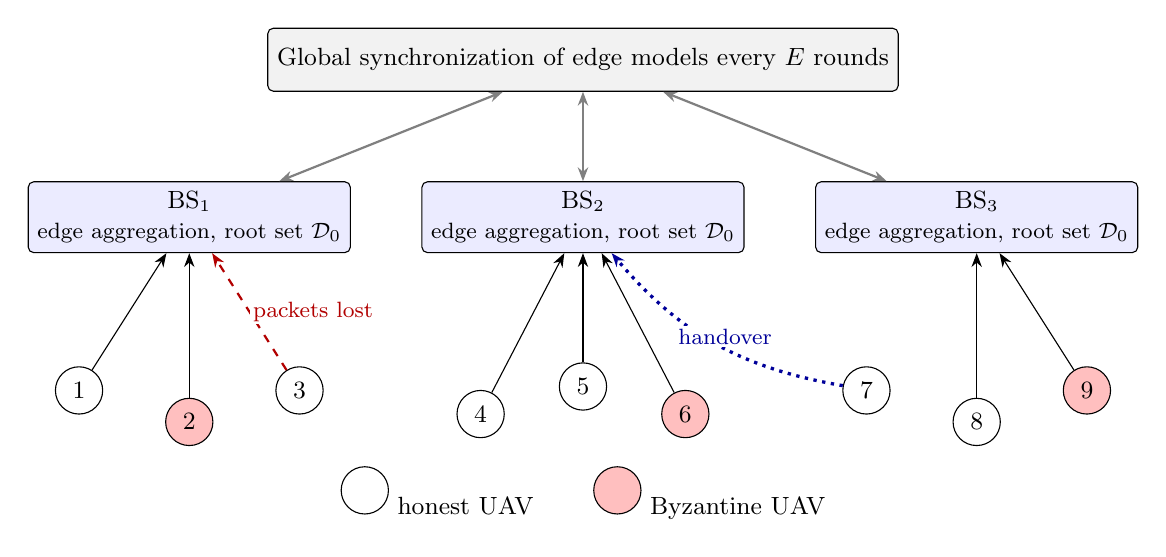
\begin{tikzpicture}[
  font=\small, >={Stealth[length=5pt]},
  bs/.style={draw, fill=blue!8, rounded corners=2pt, minimum width=20mm, minimum height=9mm, align=center},
  uav/.style={circle, draw, fill=white, inner sep=0pt, minimum size=6mm},
  bad/.style={uav, fill=red!25},
  cloud/.style={draw, fill=gray!10, rounded corners=2pt, minimum width=70mm, minimum height=8mm, align=center}]
  \node[cloud] (g) at (0,4.2) {Global synchronization of edge models every $E$ rounds};
  \foreach \x/\n in {-5/1,0/2,5/3} {
    \node[bs] (b\n) at (\x,2.2) {BS$_\n$\\{\footnotesize edge aggregation, root set $\mathcal{D}_0$}};
    \draw[<->, gray, thick] (b\n) -- (g);
  }
  \node[uav] (u1) at (-6.4,0) {1};  \node[bad] (u2) at (-5,-0.4) {2};  \node[uav] (u3) at (-3.6,0) {3};
  \node[uav] (u4) at (-1.3,-0.3) {4}; \node[uav] (u5) at (0,0.05) {5};  \node[bad] (u6) at (1.3,-0.3) {6};
  \node[uav] (u7) at (3.6,0) {7};   \node[uav] (u8) at (5,-0.4) {8};   \node[bad] (u9) at (6.4,0) {9};
  \foreach \u/\b in {1/1,2/1,4/2,5/2,6/2,8/3,9/3} \draw[->] (u\u) -- (b\b);
  \draw[->, dashed, red!70!black, thick] (u3) -- node[pos=0.5, right, fill=white, inner sep=1pt] {\footnotesize packets lost} (b1);
  \draw[->, dotted, very thick, blue!60!black] (u7) to[bend left=20] node[pos=0.45, above, fill=white, inner sep=1pt] {\footnotesize handover} (b2);
  \node at (0,-1.3) {\tikz\node[uav]{};~honest UAV \qquad \tikz\node[bad]{};~Byzantine UAV};
\end{tikzpicture}
\caption{Hierarchical FL over a UAV swarm. Each base station aggregates the updates of
the UAVs it serves, some of which arrive with lost packets; edge models are
synchronized every $E$ rounds.}
\label{fig:system}
\end{figure}

Figure~\ref{fig:system} shows the system. $K$ UAVs are served by $B$ ground base
stations (BSs). Each UAV $k$ holds a private dataset $\mathcal{D}_k$ of $n_k$ images.
In every round $t$:
\begin{enumerate}
\item each UAV attached to BS $b$ starts from that BS's edge model $\mathbf{w}^t_b$
  and trains it for one local epoch of SGD on $\mathcal{D}_k$;
\item it uploads the update $\boldsymbol{\Delta}^t_k$ (new local model minus the edge
  model), which is split into packets of $L$ parameters;
\item the BS aggregates the updates it receives and sets
  $\mathbf{w}^{t+1}_b=\mathbf{w}^t_b+\mathrm{Agg}(\cdot)$;
\item every $E$ rounds the edge models are averaged, weighted by the number of
  training samples held by the UAVs in each cell, and the result is sent back to
  every BS.
\end{enumerate}
UAVs attach to the BS with the strongest received power. A UAV hands over only when
another BS is stronger by a hysteresis margin of 3\,dB for two consecutive rounds,
which avoids ping-pong handovers (\texttt{fl/topology.py}).

\subsection{Dataset and Model}
Images come from CIFAR-10, modified to resemble aerial imagery
(\texttt{fl/data.py}). Each image is rotated by a random multiple of
$90^\circ$, since a downward-looking camera has no preferred orientation, and with
probability 0.3 or 0.2 is down-sampled to $24\times24$ or $16\times16$ pixels and
up-sampled again to imitate higher flight altitudes. The 50{,}000 training images
are split among the UAVs either uniformly (IID) or with Dirichlet($\alpha$)
class proportions; 500 images (50 per class) are held out as the trusted root set
$\mathcal{D}_0$ and are never given to any UAV.

The classifier, TacticalEdgeCNN, is a small convolutional network with about 156k
parameters and group normalization, chosen so that it could plausibly be trained on
board. Group normalization is used instead of batch normalization because batch
statistics do not average well across clients with different class mixes.

\section{Wireless Uplink Models}
\label{sec:channel}
The channel decides, for every packet of every update, whether it arrives
(\texttt{fl/channel.py}). Two models are used.

\subsection{Synthetic Jammed Channel}
UAVs move by a random walk at 100\,m altitude over an $800\times800$\,m area. The
received power from UAV $k$ at its serving BS is
\begin{equation}
  P_{\mathrm{rx},k} = P_{\mathrm{tx}} - \mathrm{PL}(d_k) + 10\log_{10}|h_k|^2,
  \qquad \mathrm{PL}(d)=40+10\eta\log_{10}d \ \text{dB},
\end{equation}
with $P_{\mathrm{tx}}=20$\,dBm, path-loss exponent $\eta=2.2$, and Rayleigh fading
$|h_k|^2\sim\mathrm{Exp}(1)$. A ground jammer of power 10\,dBm targets a sector of
the swarm, and the SINR is
\begin{equation}
  \gamma_k = P_{\mathrm{rx},k} - 10\log_{10}\bigl(N_0 + J_k\bigr),
\end{equation}
where $N_0$ corresponds to $-90$\,dBm and $J_k$ is the jamming power received at
UAV $k$'s link (zero for UAVs outside the jammed sector).

\subsection{Measured-Trace Channel}
For realism we replay a measured UAV link from DeepSense~6G
Scenario~23 \citep{alkhateeb2023deepsense,charan2025drone}, in which a drone flies
around a ground receiver that records 60\,GHz beam powers together with position,
altitude and speed. The dataset's power values are uncalibrated, so only their
variation relative to the median is used:
\begin{equation}
  \gamma_k = \bar\gamma + \bigl(P^{\mathrm{meas}}_k - \mathrm{med}\,P^{\mathrm{meas}}\bigr)
  - 10\eta\log_{10}\frac{d_{k,b}}{d_{k,1}},
\end{equation}
where $\bar\gamma$ is an assumed reference SNR and the last term adjusts the measured
link to the distance of a virtual BS $b$. Each UAV replays a different flight
segment. Two settings are used: $\bar\gamma=15$\,dB, a good link, and
$\bar\gamma=5$\,dB, a weak link. They replay identical trajectories, so only the
link quality differs.

\subsection{Packet Erasures}
In both models each packet is lost independently with probability
\begin{equation}
  p_k = \frac{1}{1+\exp\bigl(a(\gamma_k-\gamma_{\mathrm{th}})\bigr)},
\end{equation}
with $a=1$ and $\gamma_{\mathrm{th}}=3$\,dB. An update whose transmission time at
the Shannon rate exceeds the 2\,s round deadline is dropped entirely. The BS
therefore receives $\tilde{\boldsymbol\Delta}_k=\mathbf{m}_k\odot\boldsymbol\Delta_k$,
where the mask $\mathbf{m}_k$ is 1 for delivered coordinates and 0 elsewhere. The BS
also records link telemetry for each UAV: SNR, packet delivery ratio (PDR), long-run
reliability, distance, speed and handover state.

\section{Threat Model}
A fixed set of $f=3$ of the $K=10$ UAVs is Byzantine. They follow the protocol (they
train, transmit on time and use the same channel) but replace their update with one
of the following (\texttt{fl/attacks.py}, \texttt{fl/client.py}):
\begin{itemize}
\item \textbf{Label flip} (data poisoning): train on labels mapped $c\mapsto 9-c$.
\item \textbf{Sign flip}: send $-\lambda\boldsymbol\Delta_k$ with $\lambda=5$.
\item \textbf{ALIE-style} \citep{baruch2019alie}: send
  $\boldsymbol\mu-z\,\boldsymbol\sigma\odot\mathrm{sign}(\boldsymbol\mu)$ with $z=1.5$,
  where $\boldsymbol\mu$ and $\boldsymbol\sigma$ are the mean and standard deviation of
  the honest updates in the attacker's cell.
\item \textbf{IPM} \citep{xie2019ipm}: send $-\epsilon\boldsymbol\mu$ with $\epsilon=0.5$.
\end{itemize}
The ALIE and IPM attackers know the honest updates of their cell, which is a strong
assumption chosen to stress the defences. The BS's telemetry is assumed authentic;
attacks that forge it are left for Phase~II.

\section{Aggregation Rules}
All rules receive exactly the same inputs: the received updates, their masks, sample
counts and telemetry (\texttt{fl/aggregators.py}).

\subsection{Baselines}
\textbf{FedAvg} \citep{mcmahan2017fedavg} averages the received updates weighted by
$n_k$, with lost coordinates counted as zeros. \textbf{CosAvg}, the aggregation of the
earlier UAV-FL work \citep{liao2023tee} as re-implemented here, weights each update by
$\max(0,\cos(\boldsymbol\Delta_k,\bar{\boldsymbol\Delta}))\,n_k$, where
$\bar{\boldsymbol\Delta}$ is the FedAvg mean. \textbf{Coordinate-wise
median} \citep{yin2018median} takes the median of the delivered values of each
parameter. \textbf{FLTrust} \citep{cao2021fltrust} computes a root update $\mathbf{r}$
on $\mathcal{D}_0$ (with as many local steps as a typical UAV), weights each UAV by
$\max(0,\cos)$ to $\mathbf{r}$ on delivered coordinates, and rescales each update to
the norm of $\mathbf{r}$.

\subsection{Context-Calibrated Robust Aggregation (CCRA)}
CCRA is the aggregator designed in this project. Each BS applies the following
steps every round.
\begin{enumerate}
\item \textbf{Reference update.} Compute $\mathbf{r}$ on $\mathcal{D}_0$, as in FLTrust.
  Our diagnostics showed that, under non-IID data, the mean or median of the UAV
  updates is not a reliable reference: attackers and honest UAVs with skewed data
  had similar cosine similarity to it.
\item \textbf{Norm clipping.} Let $\rho_k$ be the RMS of the delivered entries of
  $\tilde{\boldsymbol\Delta}_k$ and scale the update by
  $s_k=\min(1,\ \mathrm{med}_j\rho_j/\rho_k)$, which defeats scaling attacks.
\item \textbf{Masked similarity.}
  $c_k=\cos\bigl(\mathcal{S}(s_k\tilde{\boldsymbol\Delta}_k;\mathbf{m}_k),\
  \mathcal{S}(\mathbf{r};\mathbf{m}_k)\bigr)$, where $\mathcal{S}(\cdot;\mathbf{m})$
  keeps only the coordinates with $\mathbf{m}=1$. Lost packets therefore do not make
  an honest update look dissimilar.
\item \textbf{Behaviour score.} $b_k=\mathrm{clip}\bigl(c_k/\mathrm{med}_{j:c_j>0}c_j,\
  0,\ 1\bigr)$. Updates pointing away from the reference get $b_k=0$.
\item \textbf{Reputation.} With memory $\beta$, initial trust 1 and evidence
  $e_k\in[0,1]$,
  \begin{equation}
    T_k \leftarrow T_k+\eta_k(b_k-T_k),\qquad
    \eta_k=\begin{cases}(1-\beta)\,e_k, & b_k>T_k,\\ 1-\beta, & b_k\le T_k.\end{cases}
    \label{eq:reputation}
  \end{equation}
  Penalties apply at full rate, so an attacker cannot hide by dropping its own
  packets; only rewards are slowed on poor links.
\item \textbf{Gating and averaging.} UAVs with $T_k<\tau$ are excluded. The others get
  weight $\omega_k=n_kT_k$, discounted for staleness, and each coordinate is averaged
  only over the UAVs that delivered it:
  \begin{equation}
    \mathrm{Agg}_p=\frac{\sum_k\omega_k\,m_{k,p}\,s_k\tilde\Delta_{k,p}}
                      {\sum_k\omega_k\,m_{k,p}}.
    \label{eq:masked-average}
  \end{equation}
\end{enumerate}
The evidence term multiplies five link factors:
\begin{equation}
  e_k=\mathrm{PDR}_k\cdot R_k\cdot h_k\cdot\frac{1}{1+d_k/A}\cdot\frac{1}{1+|v_k|},
\end{equation}
namely the packet delivery ratio, long-run reliability, a handover factor
($h_k=0.5$ during a handover, 1 otherwise), a distance factor with $A$ the area size,
and a normalized-speed factor.

\subsection{Ablation Variants}
To find out which part of CCRA matters, three variants are compared.
\begin{itemize}
\item \textbf{CCRA (full)}: all steps, with evidence $e_k$ from telemetry.
\item \textbf{Mask-only}: $e_k=1$, but the masks are used in steps 2--6.
\item \textbf{No-context}: $e_k=1$ and $\mathbf{m}_k=\mathbf{1}$, so lost
  coordinates enter the computation as zeros, as a channel-unaware server would see
  them.
\end{itemize}
The code also has an option to correct $c_k$ for the noise expected at the
reported SINR. It is inactive in the controlled study, which adds no residual noise
to delivered parameters, so the full-versus-mask-only contrast isolates $e_k$.

\subsection{Analysis of the Reputation Update}
\label{sec:fixed-point}
The asymmetric update~\eqref{eq:reputation} has a consequence that was not intended.
Suppose a UAV's evidence is constant, $e_k=e$, and its scores $b$ are drawn
independently from some distribution. The expected change in reputation is
\begin{equation}
  \mathbb{E}[\Delta T] = (1-\beta)\Bigl(e\,\mathbb{E}\bigl[(b-T)^+\bigr]
                        - \mathbb{E}\bigl[(T-b)^+\bigr]\Bigr),
\end{equation}
so the reputation settles where
\begin{equation}
  e\,\mathbb{E}\bigl[(b-T^\star)^+\bigr] = \mathbb{E}\bigl[(T^\star-b)^+\bigr].
  \label{eq:fixed-point}
\end{equation}
For $e=1$ the two sides balance at $T^\star=\mathbb{E}[b]$, the mean score. As $e$
decreases, the left side shrinks, and $T^\star$ must move down until few scores lie
below it; in the limit $e\to0$ it approaches the lowest score the UAV ever receives.
An honest UAV with skewed data has noisy scores, so on a weak link its reputation
tracks its worst rounds and falls below the gate $\tau$ more often. An attacker's
scores are already near zero, so slowing its rewards adds little. Section~\ref{sec:mechanism}
tests this prediction against the measured gate decisions.

\chapter{Experimental Study}
\label{ch:results}

This chapter describes how the framework was implemented and verified, the
protocol of each experiment, and the results, in the order the work was done: the
FedAvg baseline, the preliminary single-seed study, and the controlled
\NumRuns-run study, followed by a separate \BpNumRuns-run base-paper comparison.
Result tables and figures are generated from committed run-level data by the
scripts described in Appendix~B.

\section{Implementation and Verification}
Each run of the Python/PyTorch simulator saves the configuration dataclass, the
per-round history and the final model. Automated tests cover data partitioning, the
FedAvg update, attack construction, every robust aggregator, the base paper's two
erasure rules, the hierarchical server, handover logic, trace loading and the
analysis code. Review of the hierarchical simulator led to three corrections
before the controlled runs. A low delivery ratio had dampened both rewards and
penalties, so we made the penalty independent of telemetry. We also removed the
delivery-ratio input from no-context CCRA and matched the number of FLTrust root
optimizer steps to the median local step count in each cell.

\section{Experimental Protocol}
\subsection{Preliminary Study}
The preliminary runs checked the simulator end to end and provided initial
estimates of the accuracy differences. At one base station, FedAvg, the
CosAvg-style baseline and early CCRA each ran for 30 rounds with the same seed.
For each method, we crossed clean training and 30\% label flipping with ideal
delivery and synthetic jamming.

\subsection{Controlled Ablation Study}
\label{sec:protocol}
Each of the \NumSeeds{} seeds contributes 72 runs. We test FedAvg, the median,
FLTrust and three CCRA variants in every combination of the four attack settings
(clean, sign flip, ALIE and IPM) and three channels (ideal, 15\,dB trace and
5\,dB trace). For each seed we reuse the client partitions, initial weights,
attacker identities and trace positions across methods. This gives \NumRuns{}
matched runs on an NVIDIA A100.

Each run lasts 100 rounds with ten UAVs, three base stations and synchronization
every five rounds. The client partitions contain 49{,}500 images in total
($\alpha=0.5$). A separate 500 images form the trusted root set. The channels
operate without a jammer or additive noise on delivered parameters.

Before launching the runs, we specified how to measure the extra effect of
telemetry at the weaker trace anchor. For each seed, we compute the
full-minus-mask-only accuracy gap at each anchor and average the following
difference over sign flip, ALIE and IPM:
\[
  (\text{CCRA}-\text{mask-only})_{5\,\mathrm{dB}}
  -(\text{CCRA}-\text{mask-only})_{15\,\mathrm{dB}}.
\]
A practically meaningful effect requires the full 95\% interval to lie below
$-1$ point or above $+1$ point. We use percentile intervals from 10{,}000
bootstrap resamples of the paired seeds, the unit of replication. Numerical
divergence contributes 10\% accuracy, the chance level for the ten-class task.
The remaining contrasts are exploratory and use unadjusted intervals.

\subsection{Follow-up on the Base Paper's Erasure Rules}
\label{sec:bp-protocol}
For the follow-up we substitute fresh-only and reuse-old
(Section~\ref{sec:method-baselines}) for the six ablation methods. The fixed
comparison retains the original seeds, attacker identities, three channel
conditions and four attack settings. The two rules contribute 120 runs each,
for a validated total of \BpNumRuns{} outside the prespecified ablation. The
follow-up seeds were used for evaluation without parameter tuning. Both rules use the same 49{,}500 client images and reserve the same
disjoint 500 root images, although neither uses a trusted reference update.

The follow-up was executed through SwarmCompute on Windows NVIDIA workers. Final
attempts used an RTX~2060 for 238 runs and a GTX~1650 for two; 57 final attempts
resumed from centrally validated checkpoints. Configurations, source and dataset
fingerprints, terminal records and all 120 within-study scientific pairs were
checked. Runtime profiles and artifact checksums are retained with the compact
results. Hardware and software versions differ from the A100 ablation, so
cross-study rankings are descriptive. The paired fresh-only versus reuse-old
intervals resample the ten seed pairs within this follow-up; they do not make the
two studies a single prespecified experiment.

\section{FedAvg Baseline Results}
The first objective was a working FL pipeline without any defence. Ten UAVs trained
TacticalEdgeCNN for 50 rounds with two local epochs, SGD (learning rate 0.01,
momentum 0.9, batch size 64), on one BS with an ideal channel.
Table~\ref{tab:baseline} and Fig.~\ref{fig:baseline} show the result.

\begin{table}[ht]
\centering
\caption{FedAvg baseline accuracy after 50 rounds}
\label{tab:baseline}
\small
\begin{tabular}{@{}lcc@{}}
\toprule
Data partition & Final test accuracy (\%) & Best test accuracy (\%) \\
\midrule
IID (5{,}000 balanced images per UAV) & 62.6 & 62.7 \\
Non-IID, Dirichlet $\alpha=0.5$ & 60.2 & 60.6 \\
\bottomrule
\end{tabular}
\end{table}

\begin{figure}[ht]
\centering
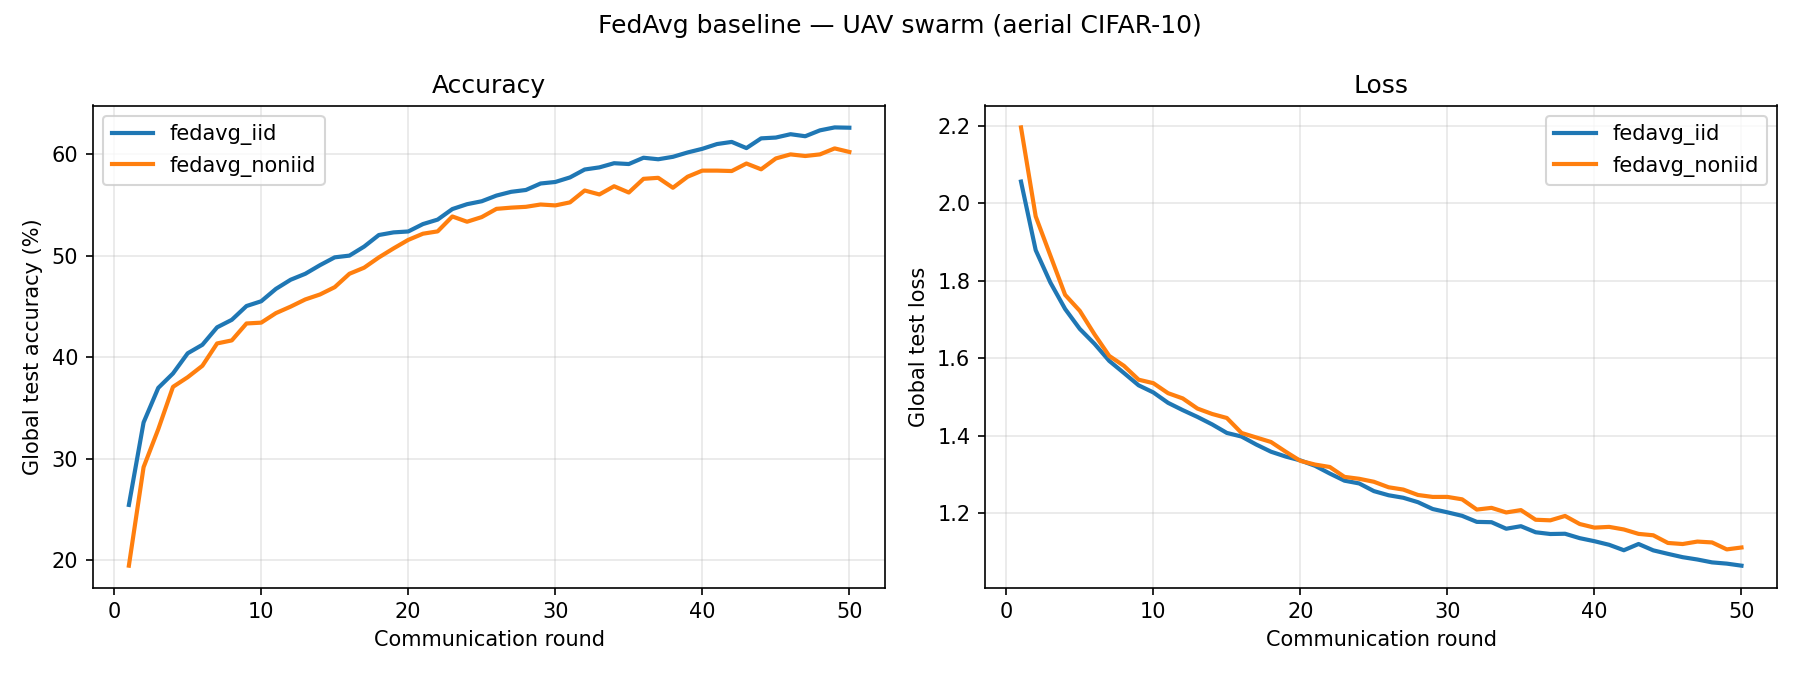
\includegraphics[width=\textwidth]{baseline_curves.png}
\caption{Test accuracy and loss of the FedAvg baseline over 50 rounds.}
\label{fig:baseline}
\end{figure}

Non-IID data cost about 2.4 percentage points, and neither curve had fully levelled
off by round 50. These accuracies are not direct targets for the later experiments,
which use 30 or 100 rounds, one local epoch and, in the controlled study, a
hierarchical system; robust methods are instead compared with matched clean controls
within each experiment.

\section{Preliminary Study Results}
The preliminary study compared FedAvg, the CosAvg-style baseline (inspired by
Liao et al.~\cite{liao2023tee}, not an exact reproduction) and an early version of CCRA with one
BS, 30 rounds, one local epoch and a single seed. Three of the ten UAVs flipped their
labels, and in the jammed scenarios a ground jammer targeted three honest UAVs.
Table~\ref{tab:prelim} lists the final accuracy (mean of the last five rounds), and
Figs.~\ref{fig:prelim-acc} and~\ref{fig:prelim-weight} show the accuracy and the
weight each method gave to the attackers.

\begin{table}[ht]
\centering
\caption{Preliminary study: final accuracy (\%), single seed, 30 rounds. CosAvg is our
CosAvg-style baseline, not the published method.}
\label{tab:prelim}
\begin{tabular}{@{}lccc@{}}
\toprule
Scenario & FedAvg & CosAvg & CCRA (early) \\
\midrule
No attack, ideal channel & 46.5 & \textbf{47.1} & 44.5 \\
No attack, jammed lossy channel & 44.6 & \textbf{45.6} & 43.1 \\
30\% label flip, ideal channel & 37.6 & 36.6 & \textbf{43.3} \\
30\% label flip, jammed lossy channel & 36.8 & 39.7 & \textbf{43.0} \\
\bottomrule
\end{tabular}
\end{table}

\begin{figure}[ht]
\centering
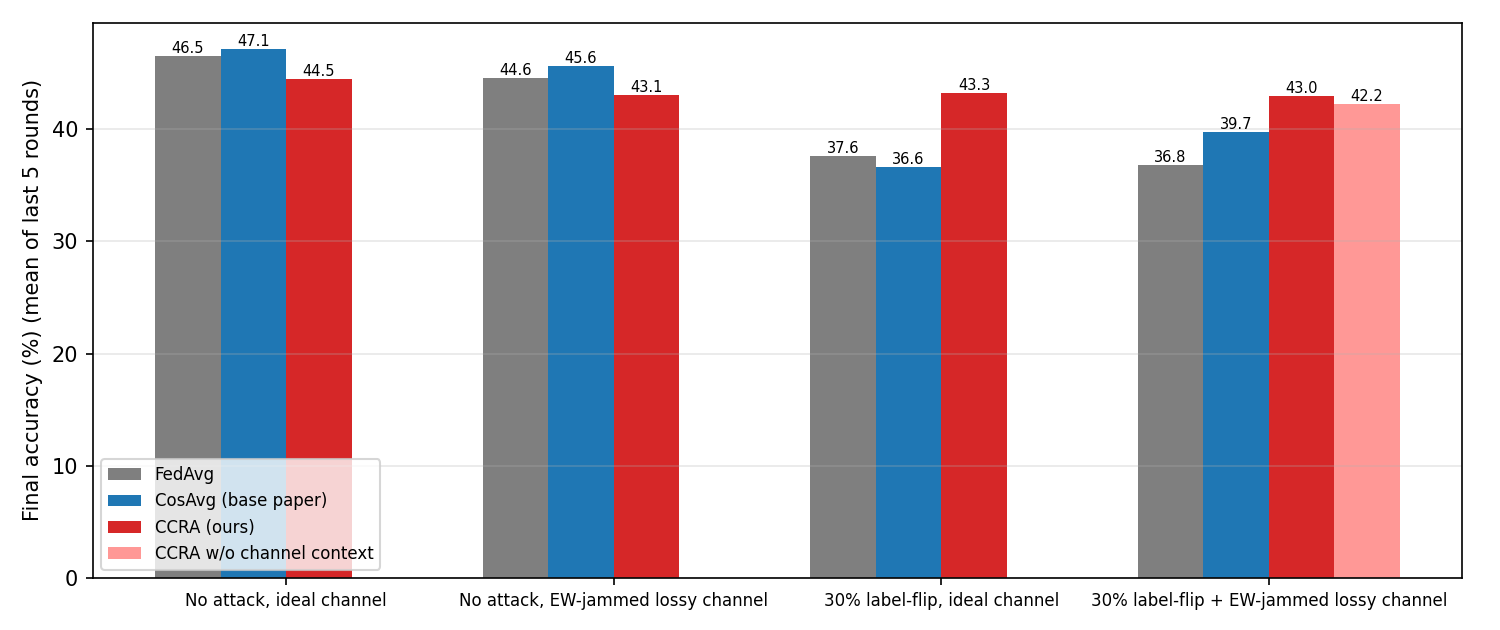
\includegraphics[width=\textwidth]{prelim_accuracy_bars.png}
\caption{Preliminary study: final accuracy in the four scenarios.}
\label{fig:prelim-acc}
\end{figure}

\begin{figure}[ht]
\centering
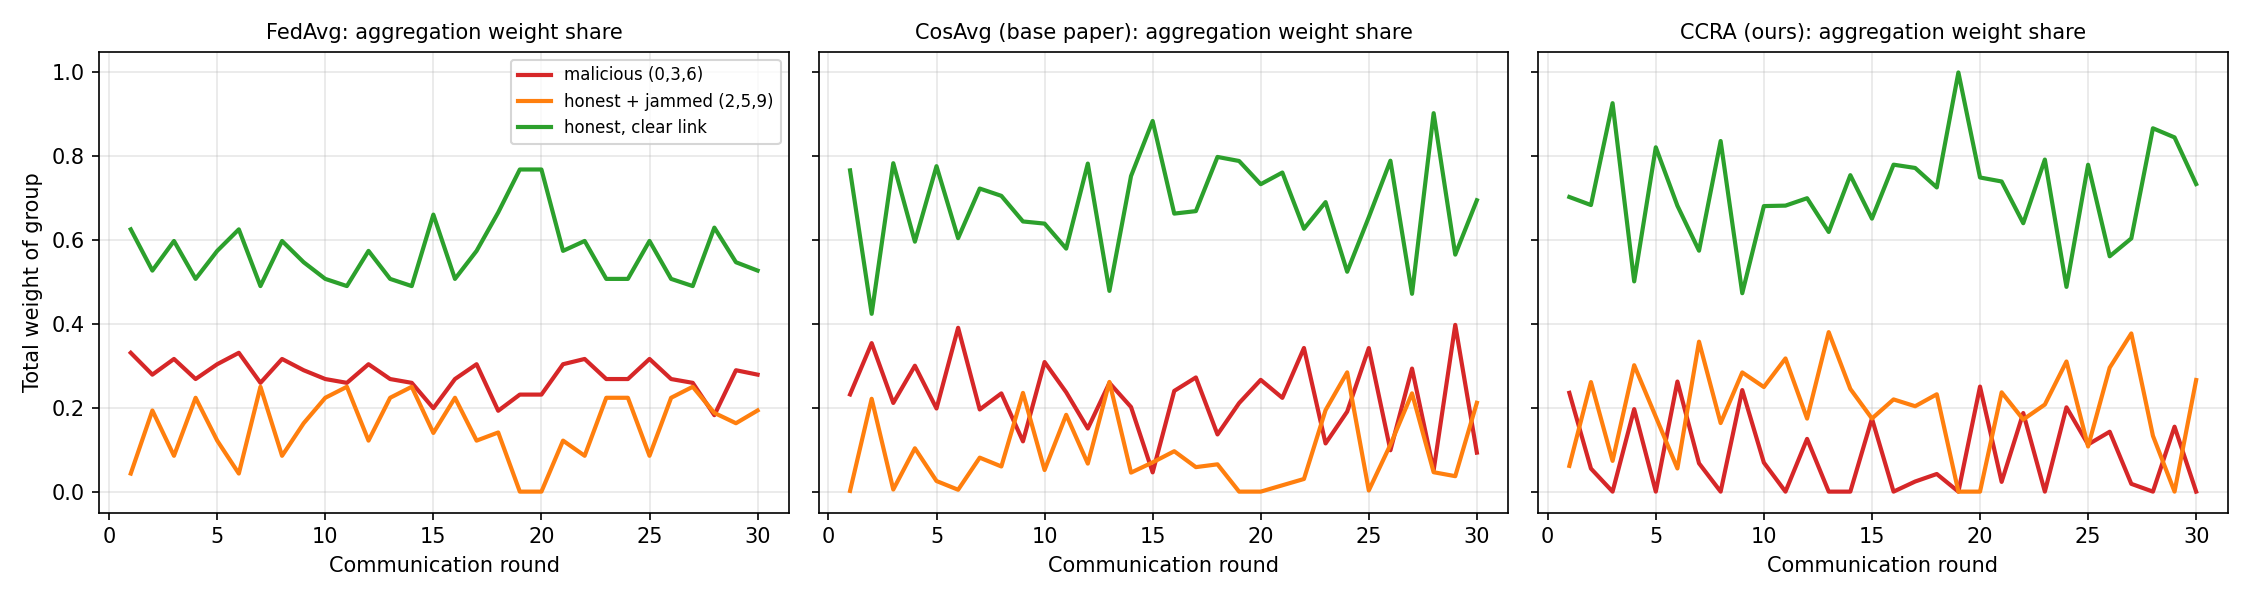
\includegraphics[width=0.9\textwidth]{prelim_weight_share.png}
\caption{Preliminary study: aggregation weight given to attackers and to jammed
honest UAVs under label flipping on the jammed channel.}
\label{fig:prelim-weight}
\end{figure}

The early CCRA kept about 43\% accuracy in both attacked scenarios. Averaged over
the last ten rounds, attackers received 1.9\% of its aggregation weight on the ideal
channel (CosAvg-style: 19.1\%; FedAvg: 26.0\%) and 8.4\% on the jammed lossy channel
(CosAvg-style: 21.5\%; FedAvg: 27.5\%). With no attack, early CCRA was 2.0 points
below FedAvg on the ideal channel and 1.5 points below it on the jammed channel;
the corresponding costs relative to the CosAvg-style baseline were 2.7 and 2.5 points.
These results were encouraging, but they could not support a claim:
\begin{itemize}
\item they came from one seed, so the size of the random variation was unknown;
\item the channel-aware part of CCRA added only 0.8 points over its no-context
  ablation (42.2 to 43.0\%), and with one seed the uncertainty in that difference
  could not be estimated;
\item CCRA used a trusted root set while CosAvg did not, so the comparison mixed two
  differences;
\item the reputation rule was revised when the system was extended to hierarchical
  FL, so the early CCRA is not the exact version evaluated in the controlled study.
\end{itemize}
The paired ablation isolates the effects of masking and telemetry.

\section{Controlled Ablation Study Results}
\label{sec:controlled}
Validation accounted for all \NumRuns{} planned outcomes, including numerical
divergences. The trace delivered on average \PdrTrace\% of packets at 15\,dB and
\PdrStress\% at 5\,dB. The two trace anchors share a geometry with neighbouring
base stations roughly 14\,m from the central station. The ideal condition instead
uses random walks and neighbours 240\,m from the centre. The change in conditions
also changes association behaviour: the ideal runs average \IdealHandovers{}
handovers, compared with \TraceHandovers{} per trace run. Comparisons with the
ideal setting therefore combine packet delivery, geometry and mobility effects.

\subsection{Stability and Overall Accuracy}
Table~\ref{tab:outcomes} pools all conditions to show divergence counts and overall
accuracy. Figure~\ref{fig:acc} restricts the accuracy comparison to attacked runs
and groups them by channel.

\begin{table}[ht]
\centering
\caption{Outcomes over all \NumRuns{} runs (120 per method). Diverged runs count as 10\%.}
\label{tab:outcomes}
\begin{tabular}{@{}lccc@{}}
\toprule
Method & Diverged & All runs (\%) & Attacked, 5\,dB (\%) \\
\midrule
FedAvg & 41/120 & 37.3 & 29.4 \\
Median & 26/120 & 29.3 & 21.3 \\
FLTrust & 0/120 & 50.6 & \textbf{50.1} \\
No-context & 0/120 & 51.4 & 45.3 \\
Mask-only & 0/120 & \textbf{52.8} & 49.5 \\
CCRA (full) & 0/120 & 51.1 & 46.0 \\
\bottomrule
\end{tabular}

\end{table}

\begin{figure}[ht]
\centering
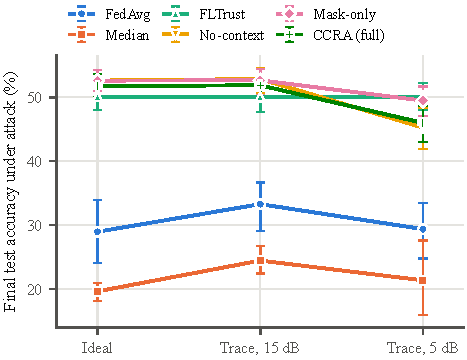
\includegraphics[width=0.75\textwidth]{accuracy_vs_channel.pdf}
\caption{Final accuracy under attack (mean over sign flip, ALIE and IPM and
\NumSeeds{} seeds). Error bars: 95\% seed-bootstrap intervals. Dashed, starred rules
are from the separate \BpNumRuns-run follow-up; cross-study rankings are descriptive.}
\label{fig:acc}
\end{figure}

FedAvg diverged in \DivFedavg{} and the coordinate-wise median in \DivMedian{} of
their 120 runs; FedAvg diverged in all 30 sign-flip runs. None of the four
methods that use a trusted reference update (FLTrust and the three CCRA variants)
diverged in its 120 runs. A plausible explanation for the median's failures, not
tested by a separate diagnostic, is that each cell holds only a few UAVs, so one
attacker in a cell is already a large fraction of the values being compared. Over all runs the mask-only variant has the highest accuracy,
\AllMask\%, against \AllFedavg\% for FedAvg. Table~\ref{tab:per-attack} breaks the
result down by attack.

\begin{table}[ht]
\centering
\caption{Final test accuracy averaged over seeds (\%). Within each attack setting,
bold marks the highest mean for each channel.}
\label{tab:per-attack}
\small
\begin{tabular}{@{}llccc@{}}
\toprule
Attack & Method & Ideal & Trace, 15 dB & Trace, 5 dB \\
\midrule
No attack & FedAvg & \textbf{59.2} & \textbf{59.3} & 54.1 \\
 & Median & 52.5 & 52.7 & 49.7 \\
 & FLTrust & 52.5 & 51.5 & 52.9 \\
 & No-context & 57.1 & 56.7 & 51.1 \\
 & Mask-only & 57.1 & 57.5 & \textbf{54.7} \\
 & CCRA (full) & 55.4 & 56.6 & 52.6 \\
\midrule
Sign flip & FedAvg & 10.0 & 10.0 & 10.0 \\
 & Median & 10.0 & 19.6 & 12.4 \\
 & FLTrust & 50.0 & 49.9 & \textbf{50.6} \\
 & No-context & \textbf{54.2} & \textbf{53.8} & 46.1 \\
 & Mask-only & 54.2 & 53.6 & 49.9 \\
 & CCRA (full) & 52.5 & 52.8 & 46.5 \\
\midrule
ALIE & FedAvg & 49.8 & 46.9 & 42.0 \\
 & Median & 35.4 & 28.4 & 28.1 \\
 & FLTrust & 49.9 & 50.6 & 49.6 \\
 & No-context & \textbf{52.9} & 52.6 & 46.0 \\
 & Mask-only & 52.9 & \textbf{52.7} & \textbf{50.8} \\
 & CCRA (full) & 52.8 & 51.9 & 46.9 \\
\midrule
IPM & FedAvg & 27.0 & 42.9 & 36.0 \\
 & Median & 13.4 & 25.3 & 23.5 \\
 & FLTrust & 50.5 & 49.7 & \textbf{50.0} \\
 & No-context & \textbf{50.7} & \textbf{52.3} & 43.6 \\
 & Mask-only & 50.7 & 51.7 & 47.7 \\
 & CCRA (full) & 50.0 & 51.0 & 44.5 \\
\bottomrule
\end{tabular}

\end{table}

Two points in Table~\ref{tab:per-attack} deserve attention. First, with no attack,
plain FedAvg is the most accurate method on the ideal and 15\,dB channels; every
robust method pays a cost of roughly two to eight points for discarding or
down-weighting honest updates. Second, on the 5\,dB channel the masked variant is
slightly ahead of FedAvg even without an attack, consistent with FedAvg's zero-filled
lost coordinates now hurting it.

\subsection{Which Kind of Channel Awareness Helps}
Figure~\ref{fig:ablation} shows the paired contrasts that separate the two channel
mechanisms.

\begin{figure}[ht]
\centering
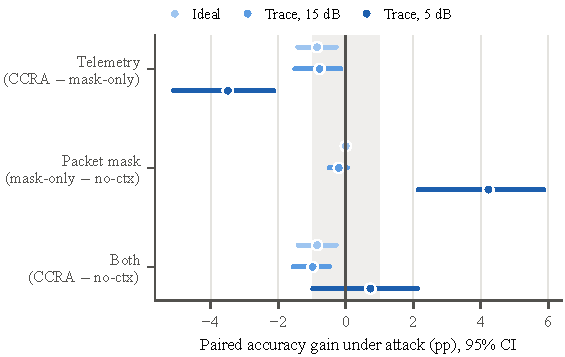
\includegraphics[width=0.75\textwidth]{ablation_contrasts.pdf}
\caption{Paired accuracy differences under attack with 95\% bootstrap intervals. The
grey band is the prespecified $\pm1$ point region of practical equivalence.}
\label{fig:ablation}
\end{figure}

\textbf{Erasure masking.} On the ideal channel nothing is lost, so mask-only and
no-context are identical. As the link weakens the masks matter more, and at 5\,dB
masking adds \MaskGain{} points over the no-context baseline, which treats lost
packets as zeros (95\% CI \ci{\MaskLo}{\MaskHi}). Treating lost
coordinates as zeros shrinks honest updates, distorts their similarity scores and
pulls the average towards zero; ignoring them avoids all three effects.

\textbf{Telemetry in the reputation.} The prespecified primary estimate, the
telemetry effect at 5\,dB minus that at 15\,dB, is $\PrimGain$ points
(\ci{\PrimLo}{\PrimHi}). Even the upper bound falls below $-1$ point, meeting the
prespecified criterion for an additional accuracy penalty at the weaker anchor.
At 5\,dB, full CCRA scored \AccCcraStress\% and mask-only scored
\AccMaskStress\%, a gap of $\TelGain$ points (\ci{\TelLo}{\TelHi}). In the
attacked ideal runs, where delivery is complete, the gap is $\TelIdeal$ points.

\textbf{Both together.} Full CCRA against no-context combines a gain and a loss; at
5\,dB the net effect is small and its interval includes the equivalence region. The
earlier impression that ``channel context helps'' came from this combination, which
hid two opposite effects.

\subsection{Mechanism: Who the Gate Rejects}
\label{sec:mechanism}
Section~\ref{sec:fixed-point} predicted that slowing rewards on weak links would push
honest UAVs' reputations down without doing much to attackers.
Figure~\ref{fig:gate} is consistent with that pattern.

\begin{figure}[ht]
\centering
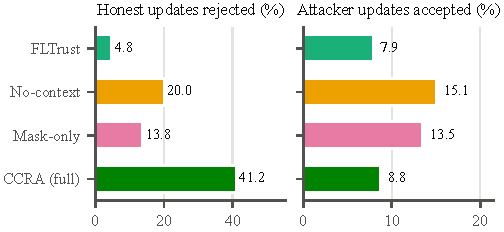
\includegraphics[width=0.75\textwidth]{gate_rates.pdf}
\caption{Gate decisions under attack at 5\,dB, as a percentage of received updates,
averaged over attacks and seeds.}
\label{fig:gate}
\end{figure}

With telemetry, the gate rejected \RejCcra\% of honest updates against \RejMask\%
without it, while the share of attacker updates accepted fell only from \AccptMask\%
to \AccptCcra\%. The accuracy loss from telemetry was accompanied by this rise in
honest-update rejection. The rule gave up a large amount of honest data to filter slightly
more attacker data, and it did so precisely when honest data were already scarce
because of packet loss. These rates are descriptive. They agree with the analysis in
Section~\ref{sec:fixed-point}, but they do not by themselves prove that it is the
cause.

\subsection{Comparison with FLTrust}
At the 5\,dB anchor under attack, FLTrust exceeds full CCRA by
\FltOverCcraStress{} points (\AccFltrustStress\% versus \AccCcraStress\%;
Table~\ref{tab:outcomes}). FLTrust is the closest established method, since it uses
the same root set, although with more root training steps. Its gate
rejected only \RejFltrust\% of honest updates at 5\,dB. It has no reputation memory,
since each round is judged on its own, but its norm matching, score normalization,
weights and gating also differ from CCRA's, so the lower rejection cannot be
attributed to memory alone. In an exploratory paired comparison, mask-only was
\VsFltTrace{} points better than FLTrust under attack at 15\,dB
(\ci{\VsFltTraceLo}{\VsFltTraceHi}), while the 5\,dB comparison was inconclusive
($\VsFltStress$ points, \ci{\VsFltStressLo}{\VsFltStressHi}): the interval supports
neither a difference nor practical equivalence, since it is not entirely inside
$\pm1$ point. The different root training budgets and aggregation rules also
limit what this comparison can establish about reputation memory.

\section{Completed Base-Paper Comparison}
\label{sec:bp-results}
The \BpNumRuns{} terminal outcomes comprise 157 successful runs and 83 numerical
divergences. Fresh-only diverged in \BpDivFresh{} of 120 runs, and reuse-old in
\BpDivReuse{} of 120. All 60 sign-flip runs diverged; the remaining 23 divergences
occurred under IPM. No clean or ALIE run diverged. These outcomes are retained at
10\% final accuracy, rather than excluded or retried into successful runs.
All-run accuracy is \BpAllFresh\% for fresh-only and \BpAllReuse\% for reuse-old.

\begin{table}[ht]
\centering
\caption{Separate base-paper follow-up: ten paired seeds per cell. Final accuracy
includes numerical divergences at chance (10\%). Intervals are exploratory paired
seed-bootstrap intervals, with no multiplicity adjustment.}
\label{tab:bp-results}
\small
\begin{tabular}{@{}llrrr@{}}
\toprule
Attack & Channel & Fresh (\%) & Reuse (\%) & Fresh $-$ reuse: pp [95\% CI] \\
\midrule
No attack & Ideal & 59.0 & 59.0 & $+0.0\;[+0.0,\,+0.0]$ \\
 & 15\,dB & 59.4 & 59.4 & $+0.0\;[-0.2,\,+0.3]$ \\
 & 5\,dB & 56.9 & 51.5 & $+5.4\;[+4.1,\,+6.7]$ \\
\midrule
Sign flip & Ideal & 10.0 & 10.0 & $+0.0\;[+0.0,\,+0.0]$ \\
 & 15\,dB & 10.0 & 10.0 & $+0.0\;[+0.0,\,+0.0]$ \\
 & 5\,dB & 10.0 & 10.0 & $+0.0\;[+0.0,\,+0.0]$ \\
\midrule
ALIE & Ideal & 49.7 & 49.5 & $+0.2\;[+0.0,\,+0.3]$ \\
 & 15\,dB & 47.2 & 47.2 & $+0.0\;[-0.3,\,+0.3]$ \\
 & 5\,dB & 43.3 & 39.8 & $+3.5\;[+0.5,\,+6.5]$ \\
\midrule
IPM & Ideal & 26.9 & 26.9 & $+0.0\;[-0.1,\,+0.0]$ \\
 & 15\,dB & 42.9 & 42.9 & $+0.0\;[-0.1,\,+0.2]$ \\
 & 5\,dB & 37.5 & 30.8 & $+6.7\;[+1.4,\,+15.0]$ \\
\bottomrule
\end{tabular}

\end{table}

Table~\ref{tab:bp-results} shows identical mean accuracy on the clean ideal channel,
where there are no missing packets to reuse. On clean stressed links, fresh-only
attains \BpCleanStressFresh\% versus \BpCleanStressReuse\% for reuse-old: a gain of
\BpCleanGain{} percentage points (95\% CI \ci{\BpCleanLo}{\BpCleanHi}). Under attack
at 5\,dB, the chance-scored means are \BpAttackStressFresh\% and
\BpAttackStressReuse\%, respectively, a gain of \BpAttackGain{} points
(\ci{\BpAttackLo}{\BpAttackHi}). The interval describes a mean over the three
attacks within each seed, not 30 independent replicates.

Retaining old parameters does not improve this finite-horizon stressed-channel
experiment, and neither rule provides Byzantine robustness. This is compatible with
the scope of Shirvanimoghaddam et al.~\cite{shirvanimoghaddam2022erroneous}: its analysis assumes honest
clients and whole-upload erasures, whereas the present implementation uses packet
erasures in a hierarchical non-IID CNN task with adversarial updates. These results
are an adaptation study, not an exact reproduction or a refutation of the original
convergence theorem.

Figure~\ref{fig:acc} now includes both rules alongside the original six methods.
The original ablation's findings about masking and telemetry are unchanged.

\subsection{Our Method against the Base Paper}
\label{sec:vs-bp}
Both studies use the same seeds, data partitions and attacker identities, so mask-only
CCRA can be compared with the base paper's better rule, fresh-only, seed by seed. Under
attack at 5\,dB, mask-only attains \AccMaskStress\% against \BpAttackStressFresh\% for
fresh-only, a paired gain of \VsBpAttack{} percentage points (95\% CI
\ci{\VsBpAttackLo}{\VsBpAttackHi}). Without attack at 5\,dB, fresh-only is ahead,
\BpCleanStressFresh\% against \AccMaskCleanStress\%, a signed difference of $\VsBpClean$ points
(\ci{\VsBpCleanLo}{\VsBpCleanHi}); the signed contrast is mask-only minus fresh-only.
FLTrust, which also uses a trusted reference, scored \FltVsBpAttack{} points
above fresh-only in the attacked 5\,dB comparison. Fresh-only already restricts
its average to delivered coordinates. Both contrasts also include differences
in scoring and weighting. The controlled comparison with zero-filled no-context
CCRA estimates the effect of masking separately.

The two studies ran on different hardware (an A100 against RTX~2060 and GTX~1650
workers) and software versions, so these contrasts are cross-study and exploratory.
Complete delivery makes fresh-only equivalent to FedAvg, giving us a cross-check
on the ideal runs. The same runs diverged in both studies. For the \XcheckRuns{}
remaining ideal pairs, the absolute accuracy difference averaged \XcheckMean{}
points and reached at most \XcheckMax{} points. This check measures agreement only
under complete delivery. The hardware contribution to the 5\,dB comparison
remains unmeasured.

The coordinator recovered interrupted jobs separately from the divergence analysis.
It verified the checkpoints before requeuing clean stops recorded as application
failures. Windows progress-file permission errors triggered bounded retries with
the same experiment settings. The audit history retains the failed attempts, and
validation accepted exactly one terminal record for each planned job. A resumed job
restores the saved training and random-generator states. Bitwise agreement between
GPUs was outside the scope of that validation.

\section{Discussion}
\subsection{What the Results Show}
\begin{enumerate}
\item FLTrust and the three CCRA variants completed all 480 runs without
  numerical divergence. The root set is one of several design choices that
  distinguish these methods from FedAvg and the median.
\item In the attacked trace runs, masking adds little at 15\,dB, where nearly
  every packet arrives. At 5\,dB, it raises accuracy by \MaskGain{} points.
  The study measured accuracy and stability. The computational and communication
  costs of masking remain unmeasured.
\item At 5\,dB, telemetry slowed trust recovery while the penalty for a low score
  stayed the same. The drift calculation in Section~\ref{sec:fixed-point} predicts
  that this asymmetry lowers equilibrium trust as evidence weakens.
\item In the erasure-rule follow-up, fresh-only gave higher accuracy at 5\,dB
  than reuse-old. Every sign-flip run diverged with either rule, even with
  packet-level erasure handling.
\end{enumerate}

\subsection{Why a Negative Result Is Useful}
The preliminary study suggested that CCRA's channel context was its key ingredient.
Had that claim been carried forward, Phase~II would have been built on a component
that harms accuracy. The prespecified design, paired seeds and chance scoring of
diverged runs made it possible to reject the claim with confidence, and the
analysis in Section~\ref{sec:fixed-point} points to the specific rule that must
change.

\subsection{Threats to Validity}
\begin{itemize}
\item \textbf{Channel realism.} The trace comes from one measured BS; the other BSs
  are virtual, and the 5 and 15\,dB anchors are assumptions, not calibrated values.
  The virtual neighbours are about 14\,m from the reference BS (about 28\,m from
  each other). In the separate 60-round channel validation, the median SNR at
  the nominal 5\,dB anchor is 8.6\,dB, not 5\,dB. There are no retransmissions.
  The trace replays average \TraceHandovers{} handovers. Comparisons with the
  ideal condition also reflect the different geometry and association patterns.
  The effect of frequent handovers in trace replay remains an open question.
\item \textbf{Scope of learning task.} The experiment uses one CNN trained on
  transformed CIFAR-10 images as a proxy for aerial imagery. The swarm size and
  attack strengths are fixed.
\item \textbf{Trust assumptions.} The simulation gives each BS access to a root
  set assumed to be clean. It leaves trusted execution and attestation to a future
  implementation.
\item \textbf{Attacker model.} The comparison assumes authentic telemetry and
  fixed poisoning strategies. An adaptive attacker that targets trust over
  multiple rounds, as studied by Liu et al.~\cite{liu2026evade}, is outside this
  design.
\item \textbf{Statistics.} Intervals reflect ten paired seeds. Secondary contrasts
  use unadjusted intervals. Phase~II confirmation requires fresh seeds.
\item \textbf{Execution environment.} The A100 ablation and Windows-worker follow-up
  used different GPU/software profiles and source fingerprints. Checkpoint recovery
  was verified, but hardware-controlled cross-study effects and runtime speedups
  were not measured.
\end{itemize}

\chapter{Conclusions and Future Scope of Study}
\label{ch:conclusions}

\section{Summary of the Work}
This project built a simulation framework for federated learning over a UAV swarm
whose updates travel over lossy air-to-ground links and in which some UAVs are
Byzantine. The framework supports hierarchical aggregation at three base stations,
handover, packet erasures from a synthetic jammed channel or a measured UAV trace,
five attacks and twelve selectable aggregation rules (FedAvg, the CosAvg-style
baseline, median, trimmed mean, Krum, Multi-Krum, FLTrust, three CCRA variants and the
base paper's two erasure rules), with automated tests. The controlled study evaluated
six methods; a separate \BpNumRuns-run follow-up evaluated the two base-paper rules.
A FedAvg
baseline was established first. A reputation-based aggregator, CCRA, was then
designed with two forms of channel awareness, erasure masking and telemetry-weighted
reputation. After a promising but inconclusive single-seed study, a prespecified,
paired study of \NumRuns{} runs separated the two forms and measured each one's
effect. The results have been written up as a manuscript in IEEE letter format.

\section{Conclusions}
\begin{enumerate}
\item Non-IID data reduced FedAvg accuracy from 62.6\% to 60.2\% in the baseline,
  and a 30\% label-flip attack reduced it by 8.9 points on the ideal channel and
  7.8 points on the jammed channel in the preliminary study (last-five-round means).
\item None of the four aggregators that judge updates against a trusted reference
  update diverged in its 120 runs (480 runs combined), whereas FedAvg and the
  coordinate-wise median diverged in \DivFedavg{} and \DivMedian{} of 120 runs each.
\item Ignoring lost coordinates instead of treating them as zeros (erasure masking)
  improved accuracy under attack on a 5\,dB link by \MaskGain{} percentage points
  (95\% CI \ci{\MaskLo}{\MaskHi}).
\item Using link telemetry to slow reputation rewards had a meaningful negative
  effect: the prespecified primary estimate was $\PrimGain$ points
  (\ci{\PrimLo}{\PrimHi}), accompanied by a rise in honest-update rejection from
  \RejMask\% to \RejCcra\%.
\item A plausible cause is structural. With slowed rewards but full-rate penalties,
  the constant-evidence drift analysis~\eqref{eq:fixed-point} shows that weaker
  evidence lowers the equilibrium of an honest UAV's reputation from its mean score
  toward the lower tail of its scores, and the measured gate decisions are
  consistent with this mechanism.
\item On weak links, the exploratory comparison of the best variant with FLTrust was
  inconclusive; a clear advantage over FLTrust appeared only at 15\,dB.
\item Against the base paper, mask-only CCRA was \VsBpAttack{} points more accurate
  than its better erasure rule under attack at 5\,dB (\ci{\VsBpAttackLo}{\VsBpAttackHi}),
  with a signed clean contrast of $\VsBpClean$ points (mask-only minus fresh-only;
  \ci{\VsBpCleanLo}{\VsBpCleanHi}). FLTrust also gains \FltVsBpAttack{} points
  over fresh-only under attack. This large gain reflects trusted-reference defence;
  our distinct findings concern masking and the telemetry rule.
\item Within the base paper's rules, fresh-only exceeds reuse-old by
  \BpCleanGain{} points on clean stressed links
  (\ci{\BpCleanLo}{\BpCleanHi}). The rules diverged in \BpDivFresh/120 and
  \BpDivReuse/120 runs; neither survived the tested sign-flip attack. This does not
  contradict the original paper's honest-client convergence analysis.
\end{enumerate}

\section{Scope for Future Work (Phase II)}
\begin{enumerate}
\item \textbf{Extend the completed base-paper comparison.} Repeat key contrasts on
  a common hardware/software stack and fresh seeds. Evaluate whether filling lost
  packets from a trusted UAV's previous parameters can improve on masking without
  retaining poisoned values.
\item \textbf{Redesign the reward rule} so that weak links do not bias reputation
  downwards, for example by making the update symmetric in the evidence, or by
  normalizing each UAV's score against its own recent history, and freeze the rule
  before testing.
\item \textbf{Confirm on fresh seeds and conditions.} Evaluate the revised rule on
  new seeds and channel settings rather than the ten used here, so that tuning
  cannot inflate the result.
\item \textbf{Mobility and handover.} Use traces or mobility models with frequent
  handovers, and more base stations, to test whether telemetry helps when the
  dominant impairment is handover rather than fading.
\item \textbf{Stronger attackers.} Add adaptive attacks that target the reputation
  itself and attackers that spoof their link telemetry.
\item \textbf{Network-level simulation.} Replace the packet-error model with a
  network simulator such as NS-3 to capture medium access, retransmissions and
  latency.
\item \textbf{Generalization.} Repeat the key comparisons with another dataset, a
  larger model and a larger swarm, and submit the manuscript.
\end{enumerate}


% References, then appendices, as in the template.
\clearpage
\phantomsection\addcontentsline{toc}{chapter}{References}
\bibliographystyle{abbrvnat}
\bibliography{refs}

% Appendices follow the references, as in the institute template.
\clearpage
\phantomsection\addcontentsline{toc}{chapter}{Appendix-A}
\chapter*{Experimental Settings}\markboth{Appendix-A}{Appendix-A}
\setcounter{table}{0}\renewcommand{\thetable}{A.\arabic{table}}
\label{app:settings}

\begin{table}[ht]
\centering
\caption{Settings of the controlled study}
\label{tab:settings}
\begin{tabularx}{\textwidth}{@{}l X@{}}
\toprule
Parameter & Value \\
\midrule
UAVs $K$, base stations $B$ & 10, 3 \\
Byzantine UAVs $f$ & 3, fixed per seed across all methods \\
Rounds; synchronization period $E$ & 100; 5 \\
Local training & 1 epoch, SGD, learning rate 0.01, momentum 0.9, batch 64, weight decay $5\times10^{-4}$ \\
Model & TacticalEdgeCNN, 156{,}074 trainable parameters, no normalization layers \\
Data & Aerial-transformed CIFAR-10, Dirichlet $\alpha=0.5$, 49{,}500 training images to UAVs \\
Root set $\mathcal{D}_0$ & 500 images (50 per class), disjoint from all UAV data \\
Reputation & $\beta=0.5$, gate $\tau=0.3$, initial trust 1 \\
Staleness discount & $\exp(-0.5\,\cdot\,\text{staleness})$; late updates dropped \\
Packets & $L=1024$ parameters, 32 bits per parameter \\
Packet errors & logistic, slope $a=1$, threshold $\gamma_{\mathrm{th}}=3$\,dB \\
Round deadline; bandwidth & 2\,s; 20\,MHz \\
Handover & 3\,dB hysteresis, 2-round time to trigger \\
Trace & DeepSense~6G Scenario~23, stride 5 samples per round, segments $\ge 200$ samples \\
Reference SNR $\bar\gamma$ & assumed anchors: 15\,dB (good link), 5\,dB (weak link) \\
Jammer; parameter noise & none; none \\
Attacks & sign flip $\lambda=5$; ALIE-style $z=1.5$; IPM $\epsilon=0.5$ \\
Seeds & 41--50 \\
\bottomrule
\end{tabularx}
\end{table}

\clearpage
\phantomsection\addcontentsline{toc}{chapter}{Appendix-B}
\chapter*{Reproducing the Results}\markboth{Appendix-B}{Appendix-B}
\setcounter{table}{0}\renewcommand{\thetable}{B.\arabic{table}}
\label{app:repro}

All code, the run-level summary results and this report are in the repository
\url{https://github.com/sasank-555/uav-swarm-fl}. The raw DeepSense~6G data are
access-controlled and must be obtained from the dataset provider; per-run model
checkpoints are kept locally and are not distributed. The training-source commit
pinned for the controlled study is recorded in
\texttt{results/CONTEXT\_STUDY\_FINAL.md}.

\begin{table}[ht]
\centering
\caption{Repository layout}
\label{tab:repo}
\begin{tabularx}{\textwidth}{@{}l X@{}}
\toprule
Path & Contents \\
\midrule
\texttt{fl/} & Simulator: data, model, client, channel, topology, attacks, aggregators, server \\
\texttt{tests/} & Automated simulator, coordinator and analysis tests \\
\texttt{run\_context\_study.py} & Plans and runs the \NumRuns-run controlled study \\
\texttt{analyze\_context\_study.py} & Prespecified analysis with paired bootstrap \\
\texttt{results/context\_study/} & Committed summary CSV and analysis of the controlled study \\
\texttt{results/context\_final/} & Local output of the final-profile reproduction command \\
\texttt{results/base\_paper\_comparison/} & Compact evidence, paired estimates and validation of the 240-run follow-up \\
\texttt{scripts/make\_paper\_figures.py} & Builds every figure, table and number in the paper and this report \\
\texttt{paper/} & Manuscript in IEEE letter format \\
\texttt{report/} & This report \\
\bottomrule
\end{tabularx}
\end{table}

Run these commands from the repository root. The final profile writes to
\path{results/context_final/}. The published compact summaries are in
\path{results/context_study/}.
\begin{lstlisting}
pip install -r requirements.txt
python prepare_data.py
python scripts/prepare_deepsense23.py /path/to/Scenario23 --out data/channel_traces/deepsense23.npz
python run_context_study.py --profile final --device cuda --parallel 4 --out-dir results/context_final
python analyze_context_study.py results/context_final
\end{lstlisting}
To rebuild figures and numbers from the committed summaries, then compile the
letter and report, use:
\begin{lstlisting}
python scripts/make_paper_figures.py
(cd paper && tectonic -X compile main.tex)
(cd report && tectonic -X compile main.tex)
\end{lstlisting}
These last three commands require no new training. To plot a fresh reproduction
instead, pass \lstinline|--csv results/context_final/context_runs.csv| to the
figure script; its default is the committed
\texttt{results/context\_study/context\_runs.csv}.

The completed base-paper follow-up uses frozen training revision
\texttt{ad06055} and the same runner with
\lstinline|--aggs bp_fresh bp_reuse|. Its full checkpoints, coordinator audit and
prepared inputs remain local. Compact publication checks source/data fingerprints,
terminal histories and all 120 paired client-partition summaries. Recompute the
follow-up intervals from the committed summary data without training:
\begin{lstlisting}
python scripts/analyze_base_paper.py --csv results/base_paper_comparison/base_paper_runs.csv
\end{lstlisting}
Then repeat the figure-generation and document-build commands above. The result
CSV records the final attempt's runtime
profile and resumed round; an attempt that resumed may include earlier work from a
different device. The source fingerprints of both studies are retained separately.


\end{document}
